\documentclass{computationtheorypaper}
\title{计算引论课程论文}
\author{冯聪}
% \includeonly{GrammarAndLanguage}
\begin{document}
%% TODO:
%% 摘要要首行缩进
%% 参考文献不够,目前只有10,需要20
%% hyperref太炫酷了,不需要
%% 逻辑流程要加强
%% 去除一些没有讲到的东西

\maketitle
\tableofcontents
\begin{abstract}
        本文回顾和总结了计算引论的内容。计算引论是一门介绍计算理论的入门课程,包含了多个子学科:
        可计算性理论,计算复杂度理论,数理逻辑,上下文无关语言以及并行计算模型。
        本课程对每一个领域解决的问题或者提出的定理或模型进行了介绍,着重介绍了其中的算法
        或推理过程,有鉴于此,本文对课程知识的回顾也从 {\itshape 领域的问题,定理和模型、算法和
        推理过程} 这几个方面进行。

\end{abstract}

\chapter*{引言}
% 背景 目的 意义
计算引论开设的背景是计算机行业知识的更新换代非常快,相比之下,
计算机基础理论就显得格外重要。
本课的目的是使学生从专业角度掌握计算机专业中计算的基本概念和原理,
培养学生的计算机专业素养,特别是从专业理论基础上,培养学生的专业思维方式和解决问题的方法,拓展学生的思考问题空间,
为系统地掌握计算机相关领域的专业知识奠定理论基础。
本课的意义是,通过本课程的学习,学生能够判断问题的难度,
并且能够具备通过建立相应的计算模型,专业地解决问题的能力,养成专业思考的能力。

\chapter{绪论}
广义说,计算是信息处理的科学名词。 狭义说,计算是指算术、代数和微积分等。
计算的科学定义是:建立模型、进行模拟、实验、验证等\cite{DBLP:books/daglib/0086373}。
上世纪初,德国大数学家希尔伯特(Hilbert)提出:
\begin{quotation}
        是否存在着一个通用过程,这个过程能用来判定任意数学命题是否成立,即,
        输入一个数学命题,在有限时间内,如果这个命题成立,得到一个证明;或如果这个命题不成立,则得到一个反例。
\end{quotation}
图灵证明了对于平面几何来说,存在这样的过程。但是,对于一般的数学命题,不存在这样的过程。

\section{计算与计算模型}

%% lambda演算的提出者church是图灵的导师,lambda演算是“图灵完备”的,并且在图灵机
%% 之前,所以列在图灵机前面。
\subsection{Lambda演算}
\def\LambdaCalculus{$\lambda$ 演算}
\def\LambdaTerm{lambda项}

\LambdaCalculus (lambda calculus)是一套从数学逻辑中发展,以变数绑定和替换规则来研究函数
如何抽象化定义、函数如何被应用以及递归的形式系统。它由数学家阿隆佐$\cdot$ 邱奇(Church, Alonzo)
在20世纪30年代首次 发表。\LambdaCalculus 作为一种应用广泛的计算模型,可以清晰的定义什么是一个可计算函数。
而任何可计算函数都能以这种形式表达和求值,它能模拟单带图灵机的计算过程;尽管如此,\LambdaCalculus
强调的是变换规则的运用,而非实现它们的具体机器。

\LambdaCalculus 可以比拟最根本订单编程语言,它包括了一条变换规则和一条将函数抽象化
定义的方式,因此普遍公认是一种更接近软件而非硬件的方式。它对函数式编程造成了很大的
影响,比如Lisp、ML语言和Haskell语言。在1936年邱奇利用\LambdaCalculus 给出了对于
判定性问题的否定:关于两个lambda运算式是否等价的命题,无法由一个\emph{通用的算法}
判断。

\LambdaCalculus 包括了构建\LambdaTerm,对\LambdaTerm 执行规约的操作。
\begin{table}[H]
        \centering
        \caption{构建\LambdaTerm 的规则}
        \begin{tabular}{|l|l|l|}
                \hline
                语法 & 名称 & 描述 \\
                \hline
                $a$ & 变量 & 表示参数或数学/逻辑值的字元或字串 \\
                \hline
                $(\lambda x.M)$ & 抽象化 & 函数定义($M$是一个\LambdaTerm)。
                变量$x$在表达式中已被绑定。\\
                \hline
                $(M N)$ & 应用 & 将函数应用与参数。$M$ 和 $N$ 是\LambdaTerm。 \\
                \hline
        \end{tabular}
\end{table}

\subsection{图灵机}
\def\TuringMathDef{(Q, \Sigma, \Gamma, \delta, q_0, q_{accept}, q_{reject})}

图灵机 \cite{doi:10.1112/plms/s2-42.1.230} (Turing machine),
又称确定型图灵机,是英国数学家艾伦·图灵于1936年提出的一种抽象计算模型,
其更抽象的意义为一种数学逻辑机,可以看作等价于任何有限逻辑数学过程的逻辑机器。

\paragraph{图灵机的正式定义}
一台\textbf{图灵机}是一个七元有序组$\TuringMathDef$ ,其中 $Q$, $\Sigma$, $\Gamma$ 都是\emph{有限集合}, 且满足:
\begin{enumerate}
        \item $Q$ 是非空有穷状态集合;
        \item $\Sigma$ 是非空有穷输入字母表,其中不包含特殊的空白符 $\epsilon$;
        \item $\Gamma$ 是非空有穷带字母表且$\Sigma \subset \Gamma$;
        \item $\epsilon \in \Gamma - \Sigma $为\emph{空白符},
                也是唯一允许出现无限次的字符;
        \item $ \delta: Q \times \Gamma \rightarrow Q \times \Gamma \times \{L,R,X\} $
                其中 $L, R$ 表示读写头是向左移还是向右移, $X$ 表示不移动;
        \item $q_0 \in Q$ 是起始状态;
        \item $q_{accept} \in Q$ 是接受状态。$q_{reject} \in Q$ 是拒绝状态,
                且$q_{reject} \neq q_{accept}$。
\end{enumerate}

图灵机$ M = \TuringMathDef $将以如下方式运作:
刚开始的时候将输入符号串$\omega = \omega_0\omega_1\cdots\omega_{n-1} \in \Sigma^{*}$
从左到右依次填在纸带的$0,1,\cdots,n-1$号格子上,其它格子保存空白 (即填空白符$\epsilon$)。
$M$的读写头指向第0号格子,$M$处于状态$q_0$。
机器开始运行后,按照转移函数$\delta$所描述的规则进行计算。例如,若当前机器状态为$q$,读写头所指
的格子中的符号为$x$,设$\delta(q,x) = (q',x',L)$,则机器进入新状态$q'$, 将读写头所
指的格子中的符号改为$x'$,然后将读写头向左移动一个格子。若在某一时刻,读写头所指的
是第0号格子,但根据转椅函数它下一步将继续向左移,这时它停在原地不动。换句话说,读写头
始终不移出纸带的边界。若某个时刻$M$根据转移函数进入了状态$q_{accept}$,则它立刻停机 并接受输入的字符串;
若在某个时刻$M$根据转移函数进入了状态$q_{reject}$,则它立刻停机并且拒绝输入的字符串。

图灵机的变体和应用以及它在计算机理论和实际中的意义将在\cref{sec:TuringMachine}中详细讨论。

\subsection{邱奇--图灵论题}
邱奇-图灵论题(Church--Turing thesis)是一个关于可计算性理论的假设。
该假设论述了关于函数特性的,可有效计算的函数值(用更现代的表述来说——在算法上可计算的)。简单来说,
邱奇-图灵论题认为``任何在算法上可计算的问题同样可由图灵机计算''。

20世纪上半叶,对可计算性进行公式化表示的尝试有:
\begin{itemize}
        \item 美国数学家阿隆佐·邱奇创建了称为\LambdaCalculus 的方法来定义函数。
        \item 英国数学家阿兰·图灵创建了可对输入进行运算的理论机器模型,现在被称为通用图灵机。
        \item 邱奇等人一起定义了一类函数,这种函数的值可使用递归方法计算。
\end{itemize}

这三个理论在直觉上似乎是等价的——它们都定义了同一类函数。因此,计算机科学家和数学家们相信,可计算性的精确定义已经出现。
邱奇--图灵论题的非正式表述说:如果某个算法是可行的,那这个算法同样可以被图灵机,以及另外两个理论所实现。

虽然这三个理论被證明是等价的,但是其中的前提假设——``能够有效计算''是一个模糊的定义。
因此,虽然这个假说已接近完全,但仍然不能由公式证明。

图灵在1936年的论文\cite{doi:10.1112/plms/s2-42.1.230}中试图通过引入图灵机来形式地展示这一想法。
在论文中,他证明了``判定性问题''是无法解决的。
\emph{几个月之前},阿隆佐·邱奇在\cite{DBLP:journals/jsyml/Church36}中证明出了一个相似的论题,
但是他采用递归函数和\LambdaCalculus 来形式地描述有效可计算性。
\LambdaCalculus 由阿隆佐·邱奇和斯蒂芬·克莱尼提出\cite{10.2307/2372027,bernays_1936},
而递归函数由库尔特·哥德尔(Kurt G\"odel)和雅克·埃尔布朗(Jacques Herbrand)提出。
这两个机制描述的是同一集合的函数,正如邱奇和克林所展示的正整数函数那样。
在听说了邱奇的建议后,图灵很快就证明了他的图灵机实际上描述的是同一集合的函数。

\subsection{\VonArch}
\def\VonNeumann{冯·诺依曼}
\def\VonArch{\VonNeumann 体系结构}

1946年,\VonNeumann 用电子器件物理实现了图灵的计算模型,建成了世界的第一台计算机。
\textbf{\VonArch}\cite{DBLP:journals/annals/Neumann93}。 (Von Neumann architecture),
又称\textbf{普林斯顿结构} (Princeton architecture),
是一种将程序指令储存器和数据存储器合并在一起的电脑设计概念结构,
依照\VonArch 设计出的计算机又称\textbf{储存程序式计算机}。

最早的计算机器仅内含固定用途的程序。现代的某些计算器依然维持了这样的设计,只能完成特定
的任务。若想改变此机器的程序,必须更改线路、更改结构甚至重新设计机器。而储存程序型
电脑的概念改变了这一切。藉由创造一组指令架构,并将所谓的运算转化为一串程序指令的执行
细节,让机器更加灵活。储存程序计算机在体系结构上主要特点有:
\begin{enumerate}
        \item    以运算单元为中心
        \item    采用存储程序原理
        \item    存储器是按地址访问、线性编址的空间
        \item    控制流由指令流产生
        \item    指令由操作码和地址码组成
        \item    数据以二进制编码
\end{enumerate}

\section{计算能力与计算效率}
一个计算模型的计算能力是用它可计算的问题类的大小来刻画的。
目前人类尚无找到其它的计算模型,其可计算的问题类超过图灵机的计算能力。
计算效率用算法的时间需求(或空间需求)来刻画。

\subsection{P与NP问题}
非定常多项式(non-deterministic polynomial,NP)时间复杂性类,或称非确定性多项式时间复杂性类,
包含了可以在多项式时间内,对一个判定性算法问题的实例,一个给定的解是否正确的算法问题。

NP是计算复杂性理论中最重要的复杂性类之一。它包含复杂性类$P$,
即在多项式时间内可以验证一个算法问题的实例是否有解的算法问题的集合;
同时,它也包含NP完全问题,即在NP中“最难”的问题。计算复杂性理论的中心问题,
$ P/NP $问题即是判断对任意的NP完全问题,是否有有效的算法,或者$NP$与$P$是否相等。

\paragraph{形式化定义}
目前常用的定义是所谓的“关系定义式”。即对于一个语言$L$,$L$在$NP$中,
那么存在多项式时间图灵机$M$,和多项式$p$使得\cite{DBLP:journals/jacm/Ladner75}:
\begin{equation*}
        x \in L \iff \exists y \in \{0,1\}_{p(|x|)}, M(x,y) = 1
\end{equation*}

\begin{figure}[H]
        \caption{NP,P,NPC问题韦恩图}
        \centering
        \includesvg[width=0.5\textwidth]{./figure/Complexity_classes.svg}
\end{figure}

\paragraph{NP完全问题}
NP完全问题(NP-Complete, NPC),是计算复杂度理论中,决定性问题的等价之一。NPC问题
是NP(非决定性多项式时间)中最难的问题。因此NP完全问题应该是最不可能被化简为P
(多项式时间可决定)的决定性问题的集合。若\emph{任何}NPC问题得到多项式时间的解法,
那此解法就可以应用在所有NP问题上。

一个决定性问题$C$若是NPC,则表示它对NP是完备的,则:
\begin{enumerate}
        \item 它是一个NP问题,且
        \item 其他属于$NP$的问题都可以\emph{规约}成它。
\end{enumerate}
\textbf{可归约} 在此表示对每个问题$L$,总有一个多项式时间多对一变换,即一个决定性的
算法可以将实例$ l \in L $转化为实例$ c \in C $,并让$c$回答Yes当且仅当此答案对$I$也是
Yes \cite{DBLP:journals/jacm/Ladner75}。
第一个NPC问题是由Leonid Levin和Cook独立证出SAT问题是NPC问題\cite{DBLP:conf/stoc/Cook71}。
此后,许多问题被陆续证明为是NP完全问题。
% 这里以后如果字数不够可以在加一些。
一些经典的NPC问题:
\begin{itemize}
        \item 布尔可满足性问题
        \item N-puzzle问题(华容道问题)
        \item 哈密尔顿圆圈问题
        \item 邮递员问题
        \item 子图同构问题
        \item 分团问题
        \item 顶点覆盖问题
        \item 独立顶点集问题
        \item 图着色问题
\end{itemize}

\begin{figure}[H]
        \caption{NPC问题的推导关系}
        \centering
        \includesvg[width=0.5\textwidth]{./figure/Relative_NPC_chart.svg}
\end{figure}

\subsection{算法分析}
在计算机科学中,算法分析(Analysis of algorithm)
是分析执行一个给定算法需要消耗的计算资源数量(例如计算时间,存储器使用等)的过程\cite{DBLP:books/daglib/0023376}。
算法的效率或复杂度在理论上表示为一个函数。其定义域是输入数据的长度(通常考虑任意大的输入,没有上界),
值域通常是执行步骤数量(时间复杂度)或者存储器位置数量(空间复杂度)。算法分析是计算复杂度理论的重要组成部分。
理论分析常常利用渐近分析估计一个算法的复杂度,并使用大$O$符号、大$\Omega$符号和大$\Theta$符号作为标记。

举例,二分查找所需的执行步骤数量与查找列表的长度之对数成正比,记为 $ O(\log n) $
简称为``对数时间''。通常使用渐近分析的原因是,同一算法的不同具体实现的效率可能有差别。
但是,对于任何给定的算法,所有符合其设计者意图的实现,它们之间的性能差异应当仅仅是一个系数。

精确分析算法的效率有时也是可行的,但这样的分析通常需要一些与具体实现相关的假设,称为计算模型。
计算模型可以用抽象机器来定义,比如图灵机。或者可以假设某些基本操作在单位时间内可完成。

假设二分查找的目标列表总共有$n$个元素。如果我们假设单次查找可以在一个时间单位内完成,
那么至多只需要 $ \log n + 1 $ 单位的时间就可以得到结果。这样的分析在有些场合非常重要。

算法分析在实际工作中是非常重要的,因为使用低效率的算法会显著降低系统性能。
在对运行时间要求极高的场合,耗时太长的算法得到的结果可能是过期或者无用的。低效率算法也会大量消耗计算资源。

\section{计算理论的地位}
计算理论奠定了一切可计算问题的基础,它对计算机可以实际求解的问题的界限进行了划定。它为理解算法的
时间和空间复杂度,提高算法的性能提供了理论支持。它也为上下文无关语言提供了理论基础,形成了各种
编程语言语法的基础。它还在早期的人工智能发挥了一定的作用。

\chapter{计算模型}
\section{图灵机}
\label{sec:TuringMachine}
图灵机$M$能够接受停机的所有输入信息串的集合就是$M$能识别的语言。       
\begin{equation*}
        L(M) = \{ \omega | q_0 \omega \vdash  xq_fy \}
\end{equation*}
如果有图灵机识别一个语言,则称该语言是图灵可识别的。又称为递归可枚举的。
如果有图灵机对所有输入都停机,则称图灵可判定。这样的语言称为图灵可判定的。简称可判定。

\paragraph{图灵机的组成}
\begin{itemize}
        \item 两端无限的线性带(读写介质)
        \item 有限的符号表(表示信息)
        \item 有限的信息处理状态
        \item 信息处理动作(静止,左、右移)
        \item 信息处理方法(规则)
\end{itemize}
\paragraph{图灵机的变形}
\begin{itemize}
        \item 多带图灵机
        \item 非确定图灵机
        \item 多指针图灵机
        \item 多维图灵机
        \item 离线图灵机
\end{itemize}
\paragraph{与图灵机等价的计算模型}
\begin{itemize}
        \item 寄存器机
        \item 波斯特系统
        \item 组合子系统
        \item 马尔可夫算法
\end{itemize}

\section{寄存器机}
在数理逻辑和理论计算机科学中,寄存器机(Register machine),
又译为暂存器机,是以类似于使用图灵机的方式使用的一类抽象机器。所有模型都是图灵等价的。

寄存器机得名于它有一个或多个``寄存器''替代了图灵机的磁带和磁头,
这个模型使用了多个唯一寻址的寄存器,每个都持有一个单一正整数。

在文献中至少可找到4个子类,下面按最原始到最类似计算机的次序列出:
\begin{itemize}
        \item 计数器机 最原始和精简的模型。
                缺乏间接寻址。指令在按照哈佛结构的有限状态机内。
        \item 指针机 计数器机和RAM模型的混合。
                比这两个模型更少共通更多抽象。指令在按照哈佛结构的有限状态机内。
        \item 随机存取机(RAM) 带有间接寻址和通常扩充的指令集。指令在按照哈佛结构的有限状态机内。
        \item 随机存取存储程序机(RASP) 带有指令在其寄存器中的RAM,类似于通用图灵机;
                因此它是冯·诺伊曼结构的一个例子。
                但是不同于计算机的是这个模型是带有有效无限个寄存器的“理想”机器。
                不像计算机甚至RISC计算机,指令集在指令数目上是非常精简的。
\end{itemize}

任何正确定义的寄存器机都是图灵等价的。计算速度严重依赖于模型细节。
寄存器机是一种与图灵机等价的,介于图灵机和实际数字计算机之间的一种抽象机。
用于分析算法效率和机器代码相关的研究。寄存器机的一般结构为:寄存器、指令集、
控制器、输入输出带和指令标号。典型的寄存器机有计数器机、指针机和RAM机以及RASP机。

\section{RAM机}
RAM(Random Access Machine)是一种为了分析算法性能而提出的近似于真实计算机的模型。
《算法导论》\cite{DBLP:books/daglib/0023376}对RAM机的描述是:
\begin{quotation}
        在RAM模型中,我们不试图去对现代计算机中很普遍的内存体系进行建模。
        即,我们不对缓存或虚拟内存进行建模。
        几个计算模型会尝试考虑内存体系的影响,这在实时计算机上的实时程序中有时很有意义。
        本书中有少量的问题会涉及内存体系的影响,但本书中的绝大部分分析将不会考虑它们。
        包含内存体系的模型要比RAM模型要复杂的多,因此它们可能较难处理。
        此外,在实际计算机中,RAM模型分析常常能对性能进行极好的预测。
\end{quotation}
所以,RAM机是一个比图灵机更贴近实际计算机,但是对实际计算机的许多方面都做了严格规定
的理想机器,它没有考虑如访问内存和磁盘的延时或者缓存的影响,而仅仅将访问一个地址的
内容规定为一个$O(1)$的操作。事实上,RAM机还对指令及其成本做了规定
\cite{DBLP:books/daglib/0023376}:
\begin{quotation}
        严格的说,我们需要精确的定义RAM模型的指令及其成本。
        但是这样做会比较单调,并且对算法设计和分析没有多大的深入。
        所以我们必须小心的不要滥用RAM模型。
        例如,如果RAM有一个进行排序的指令会怎么样?这时我们可以用一条指令进行排序。
        这样的RAM是不现实的,因为现实中的计算机没有这样的指令。
        因此,我们的方向是现实中的计算机是如何设计的。
        RAM模型的指令能够在现实中的计算机中普遍找到:
        算数(像加、减、乘、除、取余、向下取整、向上取整)、
        数据移动(加载、保存、复制)以及控制(条件和非条件分支、子程序的调用和返回)。
        每一个这样的指令要花费一个常量时间。
\end{quotation}
除了指令及其成本,RAM还规定,指令是串行执行的,没有任何并发操作\cite{DBLP:books/daglib/0023376}。
数据的类型为整数和浮点数,数据的每一个子的大小都有限制。
在RAM机器为模型的分析中,算法耗时的基本单位为步,每一步执行常量时间,这样估计出来的时间复杂度
能够独立于具体的硬件和操作系统,对现实也具有较好的指导意义。

\chapter{文法与语言}
\section{文法}
\subsection{乔姆斯基体系}
乔姆斯基体系是计算机科学中刻画形式文法表达能力的一个分类谱系,是由诺姆·乔姆斯基于1956年提出的
\cite{DBLP:journals/tit/Chomsky56}。
它包括四个层次:
\begin{itemize}
  \item 0-型文法(无限制文法或短语结构文法)包括所有的文法。该类型的文法能够产生所有可被图灵机识别的语言。
    可被图灵机识别的语言是指能够使图灵机停机的字串,这类语言又被称为递归可枚举语言。
    注意递归可枚举语言与递归语言的区别,后者是前者的一个真子集,是能够被一个总停机的图灵机判定的语言。

  \item 1-型文法(上下文相关文法)生成上下文相关语言。这种文法的产生式规则取如 $ \alpha A \beta \rightarrow \alpha \gamma \beta $
    一样的形式。这里的$A$是非终结符号,而 $\alpha$, $\beta$ 和 $\gamma$ 是包含非终结符号与终结符号的字串;
    $\alpha$, $\beta$ 可以是空串,但 $\gamma$ 必须不能是空串;这种文法也可以包含规则 $S \rightarrow \epsilon$ ,
    但此时文法的任何产生式规则都不能在右侧包含 $S$ 。这种文法规定的语言可以被线性有界非确定图灵机接受。

  \item 2-型文法(上下文无关文法)生成上下文无关语言。这种文法的产生式规则取如 $A \rightarrow \gamma$ 一样的形式。
    这里的$A$是非终结符号,$\gamma$ 是包含非终结符号与终结符号的字串。这种文法规定的语言可以被非确定下推自动机接受。
    上下文无关语言为大多数程序设计语言的语法提供了理论基础。

  \item 3-型文法(正规文法)生成正规语言。这种文法要求产生式的左侧只能包含一个非终结符号,
    产生式的右侧只能是空串、一个终结符号或者一个终结符号后随一个非终结符号;如果所有产生式的右侧都不含初始符号$S$,
    规则 $ S \rightarrow \epsilon$ 也允许出现。这种文法规定的语言可以被有限状态自动机接受,也可以通过正则表达式来获得。
    正规语言通常用来定义检索模式或者程序设计语言中的词法结构。
\end{itemize}

正规语言类包含于上下文无关语言类,上下文无关语言类包含于上下文相关语言类,上下文相关语言类包含于递归可枚举语言类。
如\cref{fig:ChomskyVenn} 所示,这里的包含都是集合的真包含关系,也就是说:存在递归可枚举语言不属于上下文相关语言类,
存在上下文相关语言不属于上下文无关语言类,存在上下文无关语言不属于正规语言类
\cite{DBLP:journals/iandc/Chomsky59a}。

\cref{tab:ChomskyModels} 总结了上述四种类型的文法的主要特点:
\begin{table}[H]
  \centering
  \caption{乔姆斯基体系}
  \label{tab:ChomskyModels}
  \begin{tabular}{|l|l|l|l|}
    \hline
    文法 & 语言 & 自动机 & 产生规则 \\
    \hline
    0-型 & 递归可枚举语言 & 图灵机 & $\alpha \rightarrow \beta$ \\
    \hline
    1-型 & 上下文有关语言 & 线性有界非确定图灵机 & $\alpha A \beta \rightarrow \alpha \gamma \beta$ \\
    \hline
    2-型 & 上下文无关语言 & 非确定下推自动机 & $A \rightarrow \gamma $ \\
    \hline
    3-型 & 正则语言 & 有限状态机 &
    {$\begin{aligned}
        A & \rightarrow aB \\
        A & \rightarrow a
    \end{aligned}$} \tabularnewline
    \hline
  \end{tabular}
\end{table}

\begin{figure}[H]
  \centering
  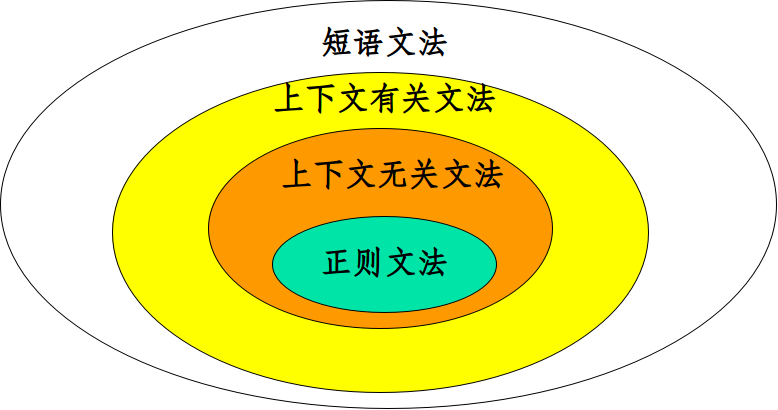
\includegraphics[width=0.68\textwidth]{figure/chomsky_model.png}
  \caption{乔姆斯基体系的韦恩图}
  \label{fig:ChomskyVenn}
\end{figure}

\section{正则文法}
\def\DFA{确定性有限自动机}
正则文法是\emph{\DFA} 识别的文法,是正则表达式的理论基础。\DFA 、正则文法和正则表达式三者是等价的。
\DFA $\mathcal{A}$ 是由:
\begin{itemize}
  \item 一个非空有限状态集合$Q$
  \item 一个输入字母表$\Sigma$(非空有限的字符集合)
  \item 一个转移函数 $ \delta: Q \times \Sigma \rightarrow Q $
    (例如: $ \delta(q, \sigma) = p, (p, q \in Q, \sigma \in \Sigma) $)
  \item 一个开始状态 $ s \in Q $
  \item 一个接受状态 $ F \subset Q $
\end{itemize}
所组成的5-元组。因此一个\DFA 可以写作这样的形式:
$ \mathcal{A} = (Q, \Sigma, \delta, s, F) $。

下面是一个\DFA 的例子。
\begin{figure}[H]
  \centering
  \includesvg[width=0.68\textwidth]{./figure/DFAexample.svg}
  \caption{\DFA 的状态图}
  \label{fig:DFAexample}
\end{figure}
\emph{正则文法} 是产生式规则取下述形式的一种形式文法$ (N, \Sigma, P, S) $:
\begin{enumerate}
  \item $A \rightarrow a$
  \item $A \rightarrow aB$
  \item $C \rightarrow \epsilon$
\end{enumerate}
此处的$A, B, C$是$N$的非终结符号,$a$是$\Sigma$中的终结符号。
这个文法描述的语言也可以用正则表达式$a^{*}bc^{*}$ 来表达。
正规文法描述的语言构成了正规语言类,
正规语言类中的语言也可以由有限状态自动机或正则表达式来表达。

\section{上下文无关文法}
\def\CFGTuple{$G = (N, \Sigma, P, S)$}
\emph{上下文无关文法}(context-free grammar,CFG),
在计算机科学中,若一个形式文法\CFGTuple 的产生式规则都取如下的形式:$V \rightarrow \omega$,其中$ V \in N, \omega \in (N \cup \Sigma)^{*} $,
则称为上下文无关文法。
上下文无关文法取名为“上下文无关”的原因就是因为字符 $V$ 总可以被字串 $\omega$ 自由替换,而无需考虑字符 $V$ 出现的上下文。
一个形式语言是上下文无关的,如果它是由上下文无关文法生成的。

上下文无关文法重要的原因在于它们拥有足够强的表达力来表示大多数程序设计语言的语法;
实际上,几乎所有程序设计语言都是通过上下文无关文法来定义的。
另一方面,上下文无关文法又足够简单,
使得我们可以构造有效的分析算法来检验一个给定字串是否是由某个上下文无关文法产生的,如LL分析器和LR分析器。

BNF(巴克斯-诺尔范式)经常用来表达上下文无关文法。

上下文无关文法$G$是4-元组:
\begin{equation*}
  G = (V, \Sigma, R, S)
\end{equation*}
\begin{enumerate}
  \item $V$ 是``非终结''符号或变量的有限集合。它们表示在句子中不同类型的
    短语或句子。
  \item $\Sigma$ 是``终结符''的有限集合,与$V$没有交集,它们构成了句子的
    实际内容。
  \item $S$是开始变量,用来表示整个句子(或程序)。它必须是$V$的元素。
  \item $R$是从$V$到$(V\cup\Sigma)^{*}$ 的关系,使得
    $ \exists \omega \in (V\cup\Sigma)^{*}: (S,\omega) \in R$。
\end{enumerate}
此外,$R$是有限集合。$R$的成员叫做文法的``规则''或者``产生式''。星号表示
\emph{Kleene星号}运算符。
例子:
\begin{lstlisting}
S ::= T '+' S | T '-' S | T
T ::= T '*' T | T '/' T | '(' S ')' | x | y | z
\end{lstlisting}
例如字符串\texttt{(x + y) * x - z * y / (x + x)}就可以用这个文法产生。

\chapter{推理与计算}

\section{逻辑与推理}
\def\PLang{\mathcal{L}}
\subsection{命题逻辑}
在逻辑和数学中,命题逻辑(或称句子逻辑)是一个形式系统,
由逻辑运算符结合原子命题来构成命题,以及允许某些公式构建成定理的一套形式证明规则。

在一阶逻辑中,命题陈述某个对象的性质,或是某些对象的关系,是能够分辨真假的语句。
一个语句如果不能再进一步分解成更简单的语句,并且又是一个命题,则称此命题为原子命题。

命题演算是一个形式系统$\PLang = \PLang(A, \Omega, Z, I)$
,它的公式如以下方式构造:
\begin{itemize}
  \item 原子命题是命题公式。
  \item 若$A$是命题公式,则$\lnot A$也是命题公式。
  \item 若$A$和$B$都是命题公式,则$A \land B$、$A \lor B$、
    $A \rightarrow B$、$A \leftrightarrow B$是命题公式。
\end{itemize}

命题公式的缺点:
\begin{itemize}
  \item 无法把所描述的客观事物的结构和逻辑特征反映出来。
  \item 不能把不同事物的共同特征反映出来。
\end{itemize}

\subsection{(一阶)谓词逻辑}
在谓词逻辑中,将原子命题分解为谓词与个体两部分。
个体是指可以独立存在的物体,可以是抽象的或具体的。
谓词则是用于刻画个体的性质、状态或个体间的关系的。
谓词的一般形式是$P(x_1, x_2, \cdots, x_n)$,其中$P$是谓词,
$x_1,x_2,\cdots,x_n$是个体。

\paragraph{项的定义:}
\begin{enumerate}
  \item 单个的常量和变量都是项。
  \item 如果$f$是函数, $t_1, \cdots, t_n$是项,那么
    $f(t_1, \cdots, t_n)$也是项。
\end{enumerate}

\paragraph{原子的定义:}
若$P$是一个$n$元谓词符号,$t_1,\cdots,t_n$是项,那么
$P(t_1,\cdots,t_n)$是原子。
\paragraph{公式的定义:}
\begin{itemize}
  \item 原子是公式。
  \item 若$P$, $Q$是公式,
    则$P \rightarrow Q$, $P \leftrightarrow Q$,
    $P \land Q$, $P \lor Q$, $\lnot P$是公式。
  \item 若$P$是公式, $x$是中的变量,则
    $\exists x P$,$\forall x P$是公式。
\end{itemize}

\paragraph{谓词公式的解释:}
设$D$为谓词公式$P$的个体域,若对$P$中的个体常量、函数和谓词按照如下规定赋值:
\begin{enumerate}
  \item 为每个个体常量指派$D$中的一个元素;
  \item 为每个$n$元函数指派一个从$D_n$到$D$的映射,其中
    \begin{equation*}
      D_n = \{ (x_1, x_2, \cdots, x_n) \  | \  x_1, x_2, \cdots, x_n \in D \}
    \end{equation*}
  \item 为每个$n$元谓词指派一个从$D_n$到$ \{F, T\} $的映射;
    则称这些指派为公式$P$在$D$上的一个解释。
\end{enumerate}

\paragraph{一阶逻辑的局限性:}
\begin{itemize}
  \item 难于表达\texttt{if-then-else}
  \item 缺乏类型的概念
  \item 难于刻画有限性或可数性
  \item 图可及性不能表达
\end{itemize}

\section{霍恩逻辑程序}
在数理逻辑中,霍恩子句(Horn Clause)是带有最多一个肯定文字的子句(文字的析取)。
霍恩子句得名于逻辑学家 Alfred Horn,
他在 1951 年首先在文章\cite{DBLP:journals/jsyml/Horn51} 中指出这种子句的重要性。

在已知的知识表示方式中,产生式表示法是一类很重要的方法,知识表示成
{\ttfamily IF ... THEN ... }的形式。霍恩子句即将规则和事实以统一的格式表示。
霍恩子句可以表示成如下形式:
\begin{equation*}
  \text{规则体} \rightarrow \text{规则头}
\end{equation*}

其中规则体一般是$n$个原子的合取, $n=0, 1, \cdots$ 。规则头可以是单个原子,也可以是空。

下面是一个霍恩子句的例子:
\begin{equation*}
  \lnot p \lor \lnot q \lor \cdots \lor \lnot t \lor u \text{,}
\end{equation*}
它可以被等价的改写为:
\begin{equation*}
  (p \land q \land \cdots \land t) \rightarrow u \text{。}
\end{equation*}

有且只有一个肯定文字的霍恩子句叫做明确子句, 没有任何肯定文字的霍恩子句叫做目标子句。
霍恩子句的合取是合取范式, 也叫做霍恩公式。
如果在一个子句中最多含有一个正文字,那么该子句称为霍恩子句。
若一个子句集内的子句个数有限且都是霍恩子句,那么该子句集称为一个霍恩逻辑程序。

霍恩子句对定理证明的实用性是一阶归结提供的,
两个霍恩子句的归结是一个霍恩子句。
在自动定理证明中,这能导致子句的在计算机上表示得更加高效。
霍恩子句在逻辑编程中扮演基本角色并且在构造性逻辑中很重要。
实际上,Prolog 就是完全在霍恩子句上构造的编程语言。
霍恩子句在计算复杂性中也是关键的,
在这里找到一组变量指派使霍恩子句的合取的为真的问题是一个P-完全问题,有时叫做 HORNSAT。
这是布尔可满足性问题的 P 的变体,它是一个中心的\emph{NP-完全问题}。

霍恩程序要素有:
\begin{enumerate}
  \item 规则: 规则体非空且规则头非空的子句。例如:
    \begin{equation*}
      father(z,y), father(y,x) \rightarrow grandfather(z,x)
    \end{equation*}
  \item 事实: 规则体空且规则头非空的子句。例如:
    $ \rightarrow father(John, Peter) $
  \item 目标: 无规则头的子句,
    例如: $ grandfather(Smith, Peter) \rightarrow\text{,} $
    即要查询$Smith$是否是$Peter$的祖父?
\end{enumerate}

一个霍恩逻辑程序是霍恩子句的集合,也就是规则和事实的集合。因此,一个霍恩逻辑程序相当于一个知识库。
推理即是通过对一组子句按照一定的方式进行消解最终得到新的公式。
自动推理的过程即给定目标子句,机器按照一定的顺序对逻辑程序中的子句进行消解,
最后得到目标子句,或者得出目标不可满足的结论。

\subsection{命题霍恩逻辑中的自动推理}
在命题霍恩逻辑中,子句之间可以按照如下的方式消解。若有子句:
\begin{align*}
  S_1 &: A_1, \cdots , A_n \rightarrow \\
  S_2 &: B_1, \cdots, B_m \rightarrow A_i
\end{align*}

则归结后的子句为:
\begin{align*}
  S_3: A_1, \cdots , A_{i-1}, \quad B_1, \cdots , B_m,
  \quad A_{i+1}, \cdots , A_n \rightarrow
\end{align*}

即利用规则$S_2$将原目标$S_1$转化为新目标$S_3$。
基于上述消解方式,求证一个目标 $ S: A_1, \cdots , A_n \rightarrow $
需要逐一以$S$的体中的每一个原子$A_i$作为新的目标进行求证。$A_1, \cdots , A_n$
也称为$S$的子目标。
在以一个原子$A_i$为目标进行求证时,考察子句集内所有头部是$A_i$的子句,
以此子句的体作为新的目标。

\cref{algo:AtomDeduce}基于上述消解方式,求证一个目标$S: A_1, \cdots, A_n \rightarrow $需要
逐一以$S$的每一个原子$A_i$作为新的目标进行求证。$A_1,\cdots,A_n$也称为
$S$的子目标。
在以一个原子$A_i$为目标进行求证时,
考察子句集内所有头部是$A_i$的子句,以此子句的体作为新的目标。
\begin{algorithm}
  \caption{原子$A$的推理算法}
  \label{algo:AtomDeduce}
  \begin{algorithmic}[1]
    \Require{$A$是原子公式}
    \Ensure{$A$是否可以消解}
    \Function{$TorF$}{$A$}
    \State $i \gets 0$
    \While{ $i < n$ } \Comment{n是此Horn逻辑程序内子句的个数}
    \If{第$i$条规则的头部$=A$} \Comment{用第$i$条规则考察$A$}
    \State\Return 1 \Comment{$A$是事实}
    \If{第i条规则的体是空的}
    \State\Return 1
    \ElsIf{$TorF(A_1) = \cdots = TorF(A_m) = 1$}\\
    \Comment{$A_1, \cdots, A_m$ 是第$i$条规则体内的所有原子}
    \State\Return 1 \Comment{由第$i$条规则推出原子$A$的正确性}
    \EndIf
    \State $i \gets i + 1$ \\
    \Comment{第$i$条规则体内并非所有原子正确,从而需要考察别的规则}
    \EndIf
    \EndWhile
    \State\Return 0 \Comment{考察了所有的规则,都不能推出$A$}
    \EndFunction
  \end{algorithmic}
\end{algorithm}

\subsection{谓词霍恩逻辑中的自动推理}

谓词Horn逻辑的消解要复杂一些。消解方式如下。若有子句:
\begin{align*}
  S_1 &: A_1 , \cdots, A_n \rightarrow \\
  S_2 &: B_1 , \cdots, B_m \rightarrow B
\end{align*}
并且$A_i, B$ 具有合一置换$\theta$,则归结后的子句为:
\begin{align*}
  S_3: (A_1, \cdots, A_{i-1}, \quad B_1, \cdots, B_m, \quad %
  A_{i+1}, \cdots, A_n) \theta \rightarrow
\end{align*}

与命题Horn逻辑相比,需要考虑项的匹配,即合一问题。
基于以上消解方式,求证一个目标$S_1:A_1, \cdots, A_n \rightarrow$ 时,
要求得出的结果应该是一个置换的集合。集合内的每一个元素$\theta_i$应该使得
$A_1\theta_i,\cdots,A_n,\theta_i$ 成立。

在以一个原子$A_i$为目标进行考察时,考察每一个头部是$A_i$的子句,
以此子句的体作为新的目标。返回的不是$0$(假)或者$1$(真),而应是一个置换的集合$\Theta$。
为此先要给出置换算法\textbf{Substitution}\cref{algo:Substitution}
以及求表达式合一算法\textbf{Unify}\cref{algo:Unify}。

\begin{algorithm}[H]
  \caption{将置换$\theta$作用于表达式$e$的算法}
  \label{algo:Substitution}
  \begin{algorithmic}[1]
    \Require{表达式$e$和置换$\theta$}
    \Ensure{$\theta$作用后的$e$}
    \Function{Substitution}{$e, \theta$}
    \If{$e$是常量符号}
    \State\Return $e$
    \EndIf
    \If{$e$是变量符号$x$}
    \If{$t/x \in \theta$}
    \State\Return $t$
    \Else
    \State\Return $e$
    \EndIf
    \EndIf
    \If{$e = f(t_1,\cdots,t_n)$}
    \State $t_1  \gets Substitution(t_1, \theta)$
    \State $\cdots$
    \State $t_n  \gets Substitution(t_n, \theta)$
    \State\Return $f(t_1,\cdots,t_n)$
    \EndIf
    \EndFunction
  \end{algorithmic}
\end{algorithm}

\begin{algorithm}[H]
  \caption{对两个表达式$e_1$,$e_2$作合一}
  \label{algo:Unify}
  \begin{algorithmic}[1]
    \Require{$e_1$,$e_2$是两个表达式}
    \Ensure{合一置换或者``无法合一''的信息}
    \Function{Unify}{$e_1, e_2$}
    \State $\theta\gets\emptyset$
    \If{$e_1$是变量符号$x$}
    \State $\theta\gets \{e_2/x\}$
    \ElsIf{$e_2$是变量符号$x$}
    \State $\theta\gets\{e_1/x\}$
    \ElsIf{$e_1$是常量而$e_2$不是 \textbf{or} $e_2$是常量而$e_1$不是%
    \textbf{or} $e_1, e_2$是两个不同的常量}
    \State\Return ``无法合一''
    \Else
    \Comment{此时$e_1,e_2$形如$f(t_1, \cdots, t_n)$
    和$g(s_1,\cdots,s_m)$;$f,g$是函数符号。}
    \EndIf
    \If{$f \neq g$}
    \State\Return ``无法合一''
    \Else
    \State $\theta_1 \gets Unify(t_1, s_1)$
    \State $\theta \gets \theta \circ \theta_1$
    \State $\theta_2 \gets Unify(Substitution(t_2, \theta), %
    Substitution(s_2,\theta))$
    \State $\theta \gets \theta \circ \theta_2$
    \State $\cdots$
    \State $\theta_n \gets Unify(Substitution(t_n, \theta), %
    Substitution(s_n, \theta))$
    \State $\theta \gets \theta_n$
    \State\Return 0
    \EndIf
    \EndFunction
  \end{algorithmic}
\end{algorithm}


\section{Prolog逻辑程序设计}
\textbf{Prolog} ({\bfseries Pro}gramming in {\bfseries Log}ic的缩写)
是一种逻辑编程语言。它建立在逻辑学的理论基础上。最初被运用于自然语言
等研究领域。现在它已广泛的应用在人工智能的研究中,它可以用来建造专家
系统、自然语言理解、智能知识库等。

\subsection*{历史}
Prolog语言最早由Aix-Marseille大学的Alain Colmerauer
与Phillipe Roussel等人于60年代末研究开发。
1972年被公认为是Prolog语言正式诞生的年份,
自1972年以后,分支出多种Prolog的方言。
最主要的两种方言为Edinburgh和Aix-Marseille。
最早的Prolog解释器由Roussel建造,而第一个Prolog编译器则是David Warren编写的。

Prolog一直在北美和欧洲被广泛使用。
日本政府曾经为了建造智能计算机而用Prolog来开发ICOT第五代计算机系统。
在早期的机器智能研究领域,Prolog曾经是主要的开发工具。

80年代Borland开发的Turbo Prolog,进一步普及了Prolog的使用。
1995年确定了ISO Prolog标准。

\subsection*{特点}
有別于一般的函数式语言,prolog的程式是基于谓词逻辑的理论。
最基本的写法是定立物件与物件之间的关系,
之后可以用询问目标的方式来查询各种物价之间的关系。
系统会自动进行匹配及回溯,找出所询问的答案。

\paragraph{执行方式}
\begin{itemize}
  \item 搜索:在程序中自上而下地搜索事实和规则;
  \item 匹配:将目标中的项与事实和规则进行匹配;
  \item 回溯:当目标中一项失败时,
    如果目标中有已经成功的的项,
    就重新调用这些成功项中的一个,谋求新的成功。
\end{itemize}

\subsection*{程序元素}
\begin{itemize}
  \item 事实:关于对象性质和关系的事实语句;
    \begin{lstlisting}[language=Prolog]
student(John), married(Tom, Mary).
human(kate).
human(bill).
likes(kate, bill).
    \end{lstlisting}

  \item 规则:关于对象性质和关系的定义规则语句;
    \begin{lstlisting}[language=Prolog]
B :- A /* 如果A则B */
    \end{lstlisting}

  \item 问题:关于对象性质或关系的询问。
    \begin{lstlisting}[language=Prolog]
?- student(John).
?- married(Mary, x).
    \end{lstlisting}
\end{itemize}

\subsection*{语法示例}
Prolog代码中以大写字母开头的元素是变量,
字符串、数字或以小写字母开头的元素是常量。下划线(\_)被称为匿名变量。
\begin{lstlisting}[language=Prolog]
/*
 * 表示kate和bill是人(human),
 * kate喜欢bill,而表示规则:
 */
friend(X, Y):-likes(X, Y), likes(Y, X).
\end{lstlisting}

\subsection{Prolog范例}
{\bfseries\raggedright 罗素悖论\par}
\begin{lstlisting}[language=Prolog]
/*
* 罗素悖论,导致不停机
*/
/* 寻找任何可以使px()规则成立的方式 */
q:- px(_).
/* 规定此规则不成立,即,此规则为假时此规则才为真 */
px(1) :- \+ px(1).
/* 启动 */
:- initialization(q).
\end{lstlisting}

\chapter*{总结}
%% 实在水不出来,哎
本文从可计算性理论,语言和文法以及推理和计算三个方面系统的阐述了
计算理论的核心问题——什么是可计算的,计算的代价如何估计,如何提供
计算的模型。计算理论为计算机的许多方面提供了理论支持,如编译原理、
密码学、操作系统、量子计算等等。计算理论中包含了一些非常简洁优雅
的证明和结论,对于提高人的逻辑思维和审美情趣有很大的帮助。



%%%
\bibliographystyle{plain}
\bibliography{paper}
\end{document}
